\begin{refsection}

	\chapter{Xarxes neuronals artificials}
	\label{chap:ANN}

	El cervell és, sens dubte, l'òrgan més complex del nostre cos. El cervell humà és una xarxa neuronal biològica: una xarxa interconnectada de neurones que transmeten senyals elèctrics. Les neurones o cèl·lules nervioses són les unitats fonamentals del cervell i el sistema nerviós. Per les \textit{dendrites} (ramificacions nervioses), les neurones reben senyals d'entrada a través dels \textit{neurotransmissors} que alliberen els \textit{axons} d'altres cèl·lules nervioses i, quan els senyals rebuts són prou forts (superen un cert \textit{llindar}), les neurones s'activen i emeten un senyal de sortida a través d'un axó. L'impuls elèctric viatja al llarg de l'axó i provoca l'alliberament de neurotransmissors en la \textit{sinapsi}, que és el punt on es produeix aquest alliberament i la recepció del missatge per una altra neurona.\supercite{ANNBeginners} D'aquesta manera les neurones es poden comunicar entre elles. Tanmateix, el funcionament del cervell humà és un misteri molt més complex, que no s'explicarà en aquest treball.

	Les xarxes neuronals artificials (en endavant, xarxes neuronals) són un model d'aprenentatge automàtic inspirat en xarxes neuronals biològiques que formen els cervells dels humans i animals. Una xarxa neuronal està formada per un conjunt d'unitats o nodes connectats anomenats neurones artificials (en endavant, neurones) que simulen el funcionament de les neurones biològiques. A través de les connexions (sinapsis en les neurones biològiques) les neurones poden transmetre i rebre senyals d'altres neurones. Cada neurona rep una sèrie d'entrades, processa aquestes entrades i emet una sortida.\supercite{ANNFundamentals}

	\section{Perceptró}

	Per començar explicaré què és un perceptró. El perceptró és la xarxa neuronal més simple possible: un model computacional duna sola neurona. Els perceptrons van ser inventats i desenvolupats en els anys 1950 i 1960 per Frank Rosenblatt.\supercite{principles} Tanmateix, el principal model de neurones més utilitzat actualment és la \textit{neurona sigmoide}.

	Un perceptró rep diverses entrades, normalment binàries, en forma de vector $\vec{x}=(x_1,x_2,\ldots,x_{n-1},x_n)$, i produeix una única sortida binària $y$. La seva funció d'activació és la funció esglaó de Heaviside (\cref{fig:heaviside}).

	\begin{figure}[h]
		\centering
		\begin{minipage}[b]{.5\textwidth}
			\centering
			\begin{tikzpicture}
				[
					cmhplot/.style={color=red,mark=none,line width=1pt,<->},
					soldot/.style={color=red,only marks,mark=*},
					holdot/.style={color=red,fill=white,only marks,mark=*}
				]
				\begin{axis}
					\addplot[cmhplot,<-,domain=-3:0]{0};
					\addplot[cmhplot,->,domain=0:3]{1};
					\addplot[soldot]coordinates{(0,1)};
					\addplot[holdot]coordinates{(0,0)};
					\node [cmhplot] at (axis cs:0,0.5) {
						$H(x) =
							\begin{cases}
								1 & \text{si $x\geq 0$} \\
								0 & \text{si $x<0$}
							\end{cases}$
					};
				\end{axis}
			\end{tikzpicture}
			\captionof{figure}{Funció esglaó de Heaviside}
			\label{fig:heaviside}
		\end{minipage}%
		\begin{minipage}[b]{.5\textwidth}
			\centering
			\begin{tikzpicture}
				[x=1.5cm, y=1.5cm, >=stealth,
					neuron/.style={
							circle,
							draw,
							minimum size=1cm
						},
				]
				\node (in-1) at (0,1.5)  {$x_1$};
				\node (in-2) at (0,0.5)  {$x_2$};
				\node [draw=none, scale=2, text height=0.333cm] (in-m) at (0,0) {$\vdots$};
				\node (in-n-1) at (0,-0.5) {$x_{n-1}$};
				\node (in-n) at (0,-1.5) {$x_n$};

				[draw=none, scale=2, text height=0.333cm] (in-m) at

				\node [neuron] (neuron) at (2,0) {$b$};

				\node (out) at (4, 0) {$f(\vec{x})$};

				\draw [->] (neuron) -- (out);

				\draw [->] (in-1) -- (neuron)
				node [above, midway] {$w_1$};
				\draw [->] (in-2) -- (neuron)
				node [above, midway] {$w_2$};
				\draw [->] (in-n-1) -- (neuron)
				node [above, midway] {$w_{n-1}$};
				%\draw [->] (in-m) -- (neuron)
				%	node [above, midway] {$\ldots$};
				\draw [->] (in-n) -- (neuron)
				node [above, midway] {$w_n$};
			\end{tikzpicture}
			\captionof{figure}{Representació d'un perceptró}
			\label{fig:perceptron}
		\end{minipage}
	\end{figure}

	En la \cref{fig:perceptron} es mostra un perceptró amb $n$ entrades. A l'hora de calcular la sortida, el vector de pesos $\vec{w}=(w_1,w_2,\ldots,w_{n-1},w_n)$ expressa la importància de les respectives entrades per a la sortida. la qual depèn de si la suma ponderada $\sum_{i=1}^{n}w_ix_i$ és major o menor que el \textit{llindar}, un paràmetre real del perceptró,\supercite{nielsen} com es pot veure en l'\cref{eq:perceptron1}:

	\begin{equation}
		\label{eq:perceptron1}
		y=f(\vec{x})=
		\begin{cases}
			1 & \text{si $\sum_{i=1}^{n}w_ix_i\geq\mathrm{llindar}$} \\
			0 & \text{altrament}
		\end{cases}
	\end{equation}

	Per simplificar podem reescriure $\sum_{i=1}^{n}w_ix_i$ com un producte escalar de vectors, $\vec{w}\cdot\vec{x}\equiv\sum_{i=1}^{n}w_ix_i$. El llindar pot ser substituït pel \textit{biaix}, $b\equiv-\mathrm{llindar}$, que indica la facilitat del perceptró per  activar-se (emetre un $1$).\supercite{TDSperceptron2} L'\cref{eq:perceptron1} es pot expressar com:

	\begin{equation}
		\label{eq:perceptron2}
		y=f(\vec{x})=
		\begin{cases}
			1 & \text{si $\vec{w}\cdot\vec{x}+b\geq0$} \\
			0 & \text{altrament}
		\end{cases}
	\end{equation}

	\begin{comment}
	\begin{figure}[h]
		\centering
		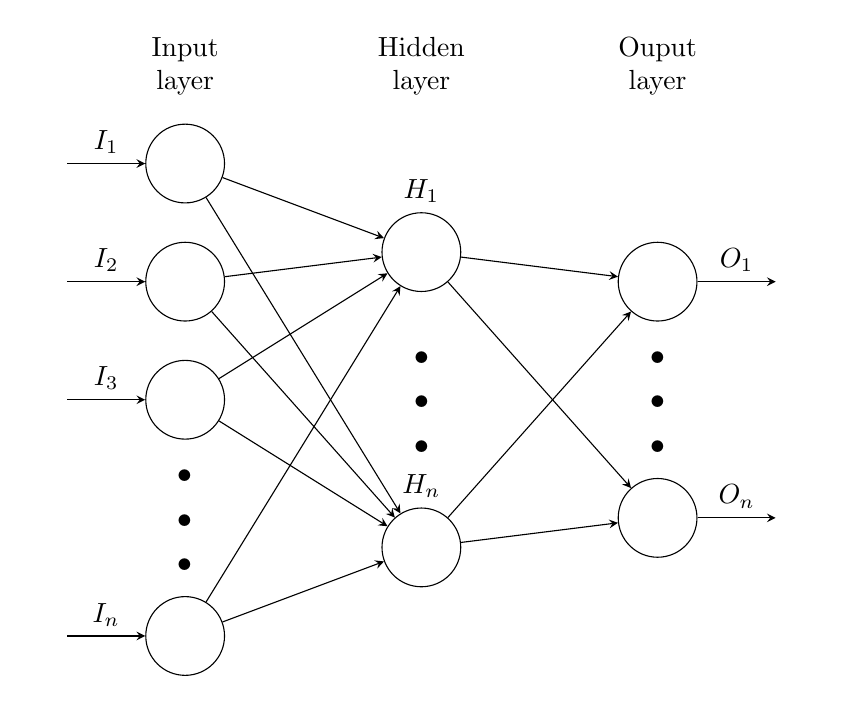
\begin{tikzpicture}
			[x=1.5cm, y=1.5cm, >=stealth,
				every neuron/.style={
						circle,
						draw,
						minimum size=1cm
					},
				neuron missing/.style={
						draw=none,
						scale=4,
						text height=0.333cm,
						execute at begin node=\color{black}$\vdots$
					},
			]

			\foreach \m/\l [count=\y] in {1,2,3,missing,4}
			\node [every neuron/.try, neuron \m/.try] (input-\m) at (0,2.5-\y) {};

			\foreach \m [count=\y] in {1,missing,2}
			\node [every neuron/.try, neuron \m/.try ] (hidden-\m) at (2,2-\y*1.25) {};

			\foreach \m [count=\y] in {1,missing,2}
			\node [every neuron/.try, neuron \m/.try ] (output-\m) at (4,1.5-\y) {};

			\foreach \l [count=\i] in {1,2,3,n}
			\draw [<-] (input-\i) -- ++(-1,0)
			node [above, midway] {$I_\l$};

			\foreach \l [count=\i] in {1,n}
			\node [above] at (hidden-\i.north) {$H_\l$};

			\foreach \l [count=\i] in {1,n}
			\draw [->] (output-\i) -- ++(1,0)
			node [above, midway] {$O_\l$};

			\foreach \i in {1,...,4}
			\foreach \j in {1,...,2}
			\draw [->] (input-\i) -- (hidden-\j);

			\foreach \i in {1,...,2}
			\foreach \j in {1,...,2}
			\draw [->] (hidden-\i) -- (output-\j);

			\foreach \l [count=\x from 0] in {Input, Hidden, Ouput}
			\node [align=center, above] at (\x*2,2) {\l \\ layer};

		\end{tikzpicture}
		\caption{Example of a parametric plot ($\sin (x), \cos(x), x$)}
	\end{figure}
	\end{comment}

	\subsection{Interpretació gràfica}
	
	\begin{figure}[H]
		\centering
		\begin{tikzpicture}
		\begin{axis}[
		axis x line=center,
		axis y line=center,
		xmin=-0.1,xmax=1.2,
		ymin=-0.1,ymax=1.2,
		xlabel=$x_1$,
		ylabel=$x_2$,
		xtick={0,1},
		ytick={0,1},
		axis on top
		]
		\addplot[name path=e,color=red,mark=none,line width=1pt,domain=-0.6:1.8]{-0.45*x+0.5};
		\node at (axis cs:0.5,0.5) {$0.9x_1+2x_2\geq1$};
		\node at (axis cs:0.3,0.1) {$0.9x_1+2x_2<1$};
		
		\addplot[name path=u,draw=none]{-0.45*x+3};
		\addplot[name path=d,draw=none]{-0.45*x-3};
		
		\addplot[color=black!10] fill between[of=e and u];
		\addplot[color=black!20] fill between[of=e and d];
		
		\end{axis}
		\end{tikzpicture}
		\caption{La separació de l'espai d'entrada amb un perceptró}
		\label{fig:separation}
	\end{figure}
	
	Un perceptró separa l'espai d'entrada en dos semiespais. Per als punts que pertanyen a un semiespai el resultat del càlcul és $0$ i per als que pertanyen a l'altre, és $1$. La \cref{fig:separation} mostra la separació del pla en dos semiplans en el cas d'un perceptró de dues entrades, $x_1$ i $x_2$, amb $\mathrm{llindar}=1$, i pesos $w_1=0.9$ i $w_2=2$. És possible generar separacions arbitràries d'espai d'entrada ajustant els paràmetres d'aquest exemple.\supercite{Rojas1996}
	
	\subsection{Exemple pràctic}
	
	En resum, un perceptró és un dispositiu que pren decisions sospesant l'evidència.\supercite{MPerceptron1,nielsen} Intentem reproduir aquest procés de presa de decisions al món real. Suposem que vull veure un partit de futbol. Abans de prendre la decisió de reservar les entrades, tindria en compte diversos factors:

	\begin{enumerate}
		\item Hi juga el meu \textit{equip} preferit?
		\item El \textit{preu} de l'entrada és barat?
		\item El \textit{temps} és bo?
	\end{enumerate}

	Aquestes són els quatre factors (variables) a partir dels quals prendré la decisió. Són les entrades binàries $x_1,x_2,x_3$ per al perceptró, respectivament. Per exemple, tenim $x_1=1$ si m'agraden els equips que juguen, i $x_1=0$ si no m'agraden. De la mateixa manera, $x_2=1$ si l'entrada és barata, i $x_2=0$ si no ho és. I de manera similar per a $x_3$.

	Ara s'ha d'establir els pesos $w_1,w_2,w_3$. Els pesos relacionen cada entrada amb la de sortida corresponent. Suposem que adoro el futbol, de manera que estic encantat d'anar al festival, encara que faci mal temps i el preu de les entrades sigui car. Però sóc molt exigent amb els equips que hi juguen.

	Podem triar un pes $w_1=6$ per als equips, i $w_2=2$ i $w_3=2$ per als altres factors (\cref{fig:experceptron}). El valor més gran de $w_1$ i indica que els equips són molt importants per a mi, molt més que el temps i el preu. També establim un llindar mitjà de 5, $\mathrm{llindar}=5$, o un biaix de -5, $b=-5$.

	Ara avaluem els dos casos següents:

	\begin{itemize}

		\item El meu equip favorit juga, $x_1=1$; el preu de l'entrada és molt alt, $x_2=0$; el temps és molt dolent, $x_3=0$. Podem veure que el valor avaluat del model és $1$, superior a $0$ (\cref{eq:case1}). Per tant, la sortida del perceptró serà $1$ (\cref{eq:perceptron1}), que vol dir que aniré al partit (\cref{fig:experceptron1}).

		      \begin{equation}
			      \label{eq:case1}
			      \vec{w}\cdot\vec{x}+b=
			      w_1x_1+w_2x_2+w_3x_3+b=
			      6\cdot1+2\cdot0+2\cdot0-5=1>0
		      \end{equation}

		\item El meu equip favorit no juga, $x_1=0$; el preu de l'entrada és molt barat, $x_2=1$; el temps és bo, $x_3=1$. Podem veure que el valor avaluat del model és $-1$, inferior a $0$ (\cref{eq:case2}). Per tant, la sortida del perceptró serà $0$ (\cref{eq:perceptron1}), que vol dir que aniré al partit (\cref{fig:experceptron2}).

		      \begin{equation}
			      \label{eq:case2}
			      \vec{w}\cdot\vec{x}+b=
			      w_1x_1+w_2x_2+w_3x_3+b=
			      6\cdot0+2\cdot1+2\cdot1-5=-1<0
		      \end{equation}

	\end{itemize}

	\begin{figure}[H]
		\centering
		\begin{subfigure}[t]{0.5\textwidth}
			\centering
			\begin{tikzpicture}
				[x=1.5cm, y=1.5cm, >=stealth,
					neuron/.style={
							circle,
							draw,
							minimum size=1cm
						},
				]
				\node (in-1) at (0,1)  {$1$};
				\node (in-2) at (0,0)  {$0$};
				\node (in-3) at (0,-1) {$0$};

				\node [neuron] (neuron) at (2,0) {$-5$};

				\node (out) at (4, 0) {$1$};

				\draw [->] (neuron) -- (out);

				\draw [->] (in-1) -- (neuron)
				node [above, midway] {$6$};
				\draw [->] (in-2) -- (neuron)
				node [above, midway] {$2$};
				\draw [->] (in-3) -- (neuron)
				node [above, midway] {$2$};
			\end{tikzpicture}
			\caption{$\vec{x}=(1,0,0)$}
			\label{fig:experceptron1}
		\end{subfigure}%
		\begin{subfigure}[t]{0.5\textwidth}
			\centering
			\begin{tikzpicture}
				[x=1.5cm, y=1.5cm, >=stealth,
					neuron/.style={
							circle,
							draw,
							minimum size=1cm
						},
				]
				\node (in-1) at (0,1)  {$0$};
				\node (in-2) at (0,0)  {$1$};
				\node (in-3) at (0,-1) {$1$};

				\node [neuron] (neuron) at (2,0) {$-5$};

				\node (out) at (4, 0) {$0$};

				\draw [->] (neuron) -- (out);

				\draw [->] (in-1) -- (neuron)
				node [above, midway] {$6$};
				\draw [->] (in-2) -- (neuron)
				node [above, midway] {$2$};
				\draw [->] (in-3) -- (neuron)
				node [above, midway] {$2$};
			\end{tikzpicture}
			\caption{$\vec{x}=(0,1,1)$}
			\label{fig:experceptron2}
		\end{subfigure}
		\caption{Exemple d'un perceptró amb $\vec{w}=(6,2,2)$ i $b=-5$}
		\label{fig:experceptron}
	\end{figure}

	Com podem veure, amb aquests paràmetres el perceptró implementa un model de presa de decisions, que produeix un $1$ a la sortida sempre que hi jugui el meu equip preferit, i un $0$ sempre que no hi jugui. El preu de les entrades i el temps no influeixen en el resultat.

	Variant els pesos i el llindar, podem obtenir diferents models de presa de decisions. Per exemple, suposem que escollim un llindar de $3$. Aleshores, el perceptró decidirà que aniré a veure el partit quan hi jugui el meu equip preferit o quan tant el preu de l'entrada sigui barat i el temps sigui bo. És a dir, seria un model diferent de presa de decisions. Un llindar més petit significa que estic més disposat a anar al partit.\supercite{nielsen}
	
	\subsection{Xarxes de perceptrons}
	
	Evidentment, el perceptró no és un model complet de presa de decisions humanes, però el que ens mostra l'exemple anterior és la capacitat d'un perceptró de prendre decisions simples. Per tant, sembla plausible que una xarxa complexa de perceptrons (\cref{fig:ann}) pugui prendre decisions molt subtils.\supercite{MPerceptron1}

	\begin{figure}[h]
		\centering
		\begin{comment}
		\begin{tikzpicture}[x=1.5cm, y=1.5cm, >=stealth,
				every neuron/.style={
					circle,
					draw,
					minimum size=1cm
				},
			]

			\foreach \m/\l [count=\y] in {1,...,4}
			\node [every neuron/.try, neuron \m/.try] (input-\m) at (0,2-\y) {$x_\m$};

			\foreach \m [count=\y] in {1,...,5}
			\node [every neuron/.try, neuron \m/.try ] (hidden1-\m) at (2,2.5-\y) {};
			
			\foreach \m [count=\y] in {1,...,4}
			\node [every neuron/.try, neuron \m/.try ] (hidden2-\m) at (4,2-\y) {};

			\foreach \m [count=\y] in {1,...,3}
			\node [every neuron/.try, neuron \m/.try ] (output-\m) at (6,1.5-\y) {};

			%\foreach \l [count=\i] in {1,2,3,n}
			%\draw [<-] (input-\l) -- ++(-1,0)
			%node [above, midway] {$x_\l$};

			%\foreach \l [count=\i] in {1,n}
			%\node [above] at (hidden1-\i.north) {$H_\l$};

			\foreach \l [count=\i] in {1,...,3}
			\draw [->] (output-\i) -- ++(1,0)
			node [above, midway] {$O_\l$};

			\foreach \i in {1,...,6n}
			\foreach \j in {1,...,5}
			\draw [->] (input-\i) -- (hidden1-\j);
			
			\foreach \i in {1,...,5}
			\foreach \j in {1,...,4}
			\draw [->] (hidden1-\i) -- (hidden2-\j);

			\foreach \i in {1,...,4}
			\foreach \j in {1,...,3}
			\draw [->] (hidden2-\i) -- (output-\j);

			\foreach \l [count=\x from 0] in {Input, Hidden, Hidden, Ouput}
			\node [align=center, above] at (\x*2,3) {\l \\ layer L_{\l+1};
		\end{tikzpicture}
		\end{comment}
		
		\begin{neuralnetwork}[height=4,nodesize=1cm,nodespacing=1.5cm,layertitleheight=5em]
			\newcommand{\nodetextclear}[2]{}
			\newcommand{\nodetextx}[2]{$x_#2$}
			\newcommand{\nodetexty}[2]{$y_#2$}
			\inputlayer[count=4, bias=false, title={Capa\\d'entrada $L_1$}, text=\nodetextx]
			\hiddenlayer[count=5, bias=false, title={Capa\\oculta $L_2$}, text=\nodetextclear] \linklayers
			\hiddenlayer[count=5, bias=false, title={Capa\\oculta $L_3$}, text=\nodetextclear] \linklayers
			\outputlayer[count=3, title={Capa\\de sortida $L_4$}, text=\nodetexty] \linklayers
		\end{neuralnetwork}
		
		\caption{Xarxa de perceptrons}
		\label{fig:ann}
	\end{figure}

	Les entrades $x_1,x_2,\ldots$ es poden representar com a variables flotant a l’esquerra de la xarxa de perceptrons (\cref{fig:perceptron}), però és convencional dibuixar una capa addicional de perceptors (la capa d’entrada $L_1$, \cref{fig:ann}) per codificar les entrades. Els perceptrons d'entrada realment no són perceptrons, sinó unitats especials que simplement emeten els valors desitjats $x_1,x_2,\ldots$.
	
	\subsection{Aprenentage del perceptró}
	
	Ara ens podem fer dues preguntes senzilles:
	
	\begin{itemize}
		\item Com seleccionar els valors dels pesos? Als exemples anteriors, aquests valors s'introdueixen manualment, però les xarxes neuronals no funcionen d'aquesta manera.
		
		\item Com seleccionar el valor del llindar o del biaix?
	\end{itemize}

	Es poden dissenyar \textit{algoritmes d'aprenentatge} que puguin ajustar automàticament els pesos i els biaixos d'una xarxa de neurones artificials. Aquest ajustament es produeix en resposta als estímuls externs, sense intervenció directa d'un programador. Els algoritmes d'aprenentatge permeten a les xarxes neuronals aprendre a resoldre problemes. Però, com podem elaborar aquests algoritmes?
	
	Suposem que tenim una xarxa de perceptors que volem utilitzar per aprendre a resoldre algun problema. Per exemple, les entrades a la xarxa poden ser els píxels d'una imatge manuscrita d'un dígit. I volem que la xarxa aprengui els pesos i els biaixos per obtenir a la seva sortida una classificació correcta del dígit. Per veure com pot funcionar l'aprenentatge, suposem que fem un petit canvi en algun pes (o biaix) a la xarxa. El que volem és que aquest petit canvi de pes causi només un petit canvi corresponent en la sortida de la xarxa (\cref{fig:learn}). Aquesta propietat farà possible l'aprenentatge.
	
	\begin{figure}[h]
		\centering
		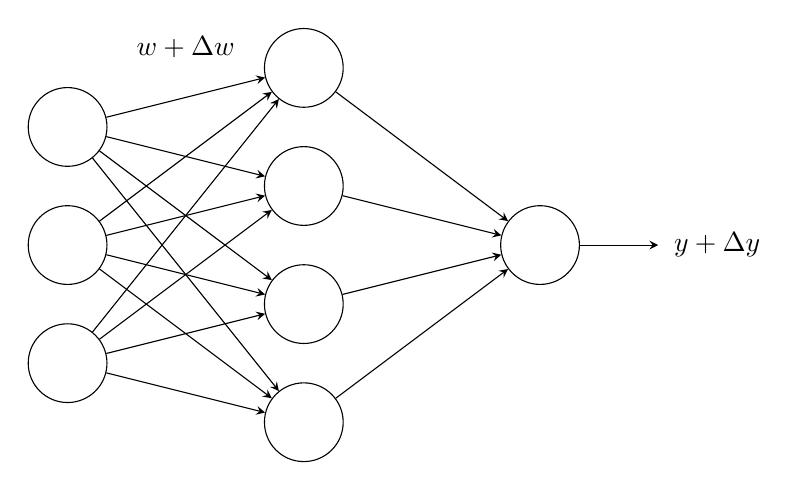
\begin{tikzpicture}[x=1.5cm, y=1.5cm, >=stealth,
			every neuron/.style={
				circle,
				draw,
				minimum size=1cm
			},
		]
			\foreach \m/\l [count=\y] in {1,...,3}
			\node [every neuron/.try, neuron \m/.try] (input-\m) at (0,2-\y) {};
		
			\foreach \m [count=\y] in {1,...,4}
			\node [every neuron/.try, neuron \m/.try ] (hidden1-\m) at (2,2.5-\y) {};
		
			\foreach \m [count=\y] in {1}
			\node [every neuron/.try, neuron \m/.try ] (output-\m) at (4,1-\y) {};
		
			%\foreach \l [count=\i] in {1,2,3,n}
			%\draw [<-] (input-\l) -- ++(-1,0)
			%node [above, midway] {$x_\l$};
		
			%\foreach \l [count=\i] in {1,n}
			%\node [above] at (hidden1-\i.north) {$H_\l$};
		
			\foreach \l [count=\i] in {1}
			\draw [->] (output-\i) -- ++(1,0);
			
			\node [align=center] at (5.5,0) {$y+\Delta y$};
		
			\foreach \i in {1,...,3}
			\foreach \j in {1,...,4}
			\draw [->] (input-\i) -- (hidden1-\j);
			
			\foreach \i in {1,...,4}
			\foreach \j in {1}
			\draw [->] (hidden1-\i) -- (output-\j);
			
			%\foreach \l [count=\x from 0] in {Input, Hidden, Ouput}
			%\node [align=center, above] at (\x*2,2.5) {\l \\ layer};
			\node [align=center, above] at (1,1.5) {$w+\Delta w$};
		\end{tikzpicture}
		\caption{Aprentatge d'una xarxa de perceptrons}
		\label{fig:learn}
	\end{figure}

	Si és cert que un petit canvi en un pes (o biaix) provoca només un petit canvi en la sortida, podem utilitzar aquest fet per modificar els pesos i els biaixos per aconseguir que la xarxa es comport de la manera que desitgem. Per exemple, suposem que la xarxa classificava erròniament una imatge com a $8$ quan hauria de ser un $9$. Podríem esbrinar com es pot fer un petit canvi en els pesos i els biaixos, de manera que la xarxa s'acosti una mica més a la correcta classificació de la imatge. I després repetiríem això, canviant els pesos i els biaixos una vegada darrere l'altra per aconseguir cada cop millors resultats. La xarxa estaria aprenent.
	
	El problema és que això no passa amb perceptrons. Així doncs, un petit canvi en els pesos o biaixos d'un sol perceptró d'una xarxa fa que la sortida d'aquesta passi de $0$ a $1$ i viceversa, canviant el comportament de la xarxa de forma molt aleatòria, ja que el perceptró replica una funció esglaó (\cref{fig:heaviside}). Això fa que sigui difícil veure com modificar gradualment els pesos i els biaixos de manera que la xarxa s’acosti al comportament desitjat.
	
	Podem superar aquest problema introduint un nou tipus de neurona artificial anomenada \textit{neurona sigmoide}.
	
	\section{Neurona sigmoide}
	
	Les neurones sigmoides són similars als perceptrons, però es modificades de tal manera que els petits canvis en els seus pesos i biaixos causen només un petit canvi en la seva sortida. Aquest fet permetrà aprendre a una xarxa de neurones sigmoides.\supercite{TDSsigmoid}
	
	Les neurones sigmoides es representen de la mateixa manera que els perceptrons (\cref{fig:neuron}).
	
	\begin{figure}[h]
		\centering
		\begin{tikzpicture}
		[x=1.5cm, y=1.5cm, >=stealth,
		neuron/.style={
			circle,
			draw,
			minimum size=1cm
		},
		]
		\node (in-1) at (0,1.5)  {$x_1$};
		\node (in-2) at (0,0.5)  {$x_2$};
		\node [draw=none, scale=2, text height=0.333cm] (in-m) at (0,0) {$\vdots$};
		\node (in-n-1) at (0,-0.5) {$x_{n-1}$};
		\node (in-n) at (0,-1.5) {$x_n$};
		
		[draw=none, scale=2, text height=0.333cm] (in-m) at
		
		\node [neuron] (neuron) at (2,0) {$b$};
		
		\node (out) at (4, 0) {$f(\vec{x})$};
		
		\draw [->] (neuron) -- (out);
		
		\draw [->] (in-1) -- (neuron)
		node [above, midway] {$w_1$};
		\draw [->] (in-2) -- (neuron)
		node [above, midway] {$w_2$};
		\draw [->] (in-n-1) -- (neuron)
		node [above, midway] {$w_{n-1}$};
		%\draw [->] (in-m) -- (neuron)
		%	node [above, midway] {$\ldots$};
		\draw [->] (in-n) -- (neuron)
		node [above, midway] {$w_n$};
		\end{tikzpicture}
		\captionof{figure}{Representació d'una neurona sigmoide}
		\label{fig:neuron}
	\end{figure}

	Igual que un perceptró, la neurona sigmoide té diverses entrades reals, $x_1,x_2,\ldots$, pesos per a cada entrada, $w_1,w_2,\ldots$ i un biaix, $b$. Però la seva sortida no és binària ($0$ o $1$). En canvi, la sortida d'una neurona sigmoide és $\sigma(\vec{w}\cdot\vec{x}+b)$, on $\sigma$ s'anomena \textit{funció sigmoide} (\cref{eq:sigmoid}, \cref{fig:sigmoid}). La funció $\sigma$ també es diu \textit{funció logística} i les neurones es diuen \textit{neurones logístiques}.
	
	\begin{equation}
		\label{eq:sigmoid}
		\sigma(x)=\frac{1}{1+e^{-x}}
	\end{equation}
	
	\begin{figure}[H]
		\centering
	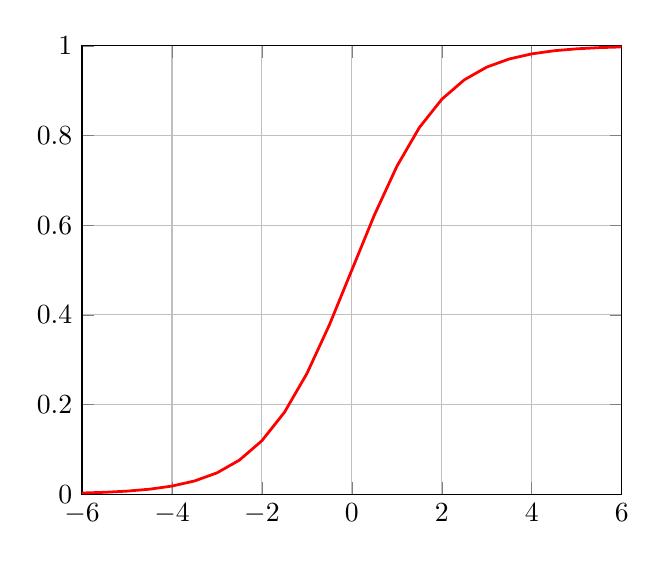
\begin{tikzpicture}
	[
	cmhplot/.style={color=red,mark=none,line width=1pt},
	]
	\begin{axis}[
	grid=both,
	xmin=-6,xmax=6,
	ymin=0,ymax=1
	]
	\addplot[cmhplot,domain=-6:6]{1/(1+exp(-x))};
	%\node [cmhplot] at (axis cs:0,0.5) {
	%	$H(x) =
	%	\begin{cases}
	%	1 & \text{si $x\geq 0$} \\
	%	0 & \text{si $x<0$}
	%	\end{cases}$
	%};
	\end{axis}
	\end{tikzpicture}
	\captionof{figure}{Funció sigmoide}
	\label{fig:sigmoid}
	\end{figure}

	En aquest cas, la funció sigmoide és la \textit{funció d'activació} o \textit{funció de transferència} de la neurona sigmoide. En el cas del perceptró, la seva funció d'activació és la funció esglaó $H(x)$ i la sortida $f(\vec{x})=H(\vec{w}\cdot\vec{x}+b)$. Per a qualsevol altra funció d'activació $g(x)$ la sortida de la neurona serà $f(\vec{x})=g(\vec{w}\cdot\vec{x}+b)$.

	Per tant, la sortida d'una neurona sigmoide amb entrades $\vec{x}=(x_1,x_2,\ldots)$, pesos $\vec{w}=(w_1,w_2,\ldots)$ i biaix $b$ és:
	
	\begin{equation}
		\label{eq:out}
		f(\vec{x})=\sigma(\vec{w}\cdot\vec{x}+b)=\frac{1}{1+e^{-(\vec{w}\cdot\vec{x}+b)}}
	\end{equation}

	La forma de la funció sigmoide (\cref{fig:sigmoid}) és una versió suavitzada de la funció esglaó (\cref{fig:heaviside}). La suavitat de $\sigma$ significa que petits canvis $\Delta w_i$ en els pesos i $\Delta b$ en el biaix produiran un petit canvi $\Delta y$ en la sortida de la neurona, propietat necessària perquè la xarxa pugui aprendre.
	
	\addtocontents{toc}{\vspace{1em}}

	\printbibliography[heading=subbibintoc]

\end{refsection}
